% fig_alpha50_vs_Irest.tex
% α₅₀ vs I_rest: fixed threshold (TR-15) vs adaptive k=0.15 for ag and 3ph
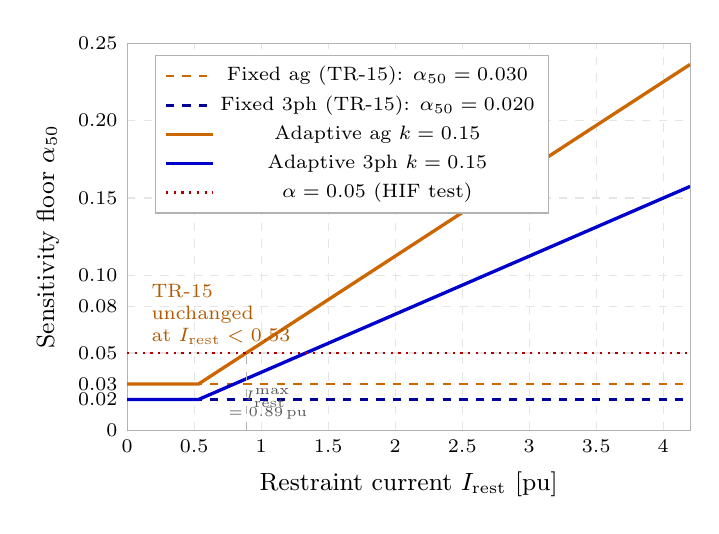
\begin{tikzpicture}
\begin{axis}[
  name        = a50ax,
  width       = 0.72\textwidth,
  height      = 6.5cm,
  xlabel      = {Restraint current $I_{\rm rest}$ [pu]},
  ylabel      = {Sensitivity floor $\alpha_{50}$},
  xlabel style= {font=\small},
  ylabel style= {font=\small},
  xmin=0, xmax=4.2,
  ymin=0, ymax=0.25,
  xtick       = {0,0.5,1,1.5,2,2.5,3,3.5,4},
  ytick       = {0,0.02,0.03,0.05,0.08,0.10,0.15,0.20,0.25},
  yticklabels = {0,0.02,0.03,0.05,0.08,0.10,0.15,0.20,0.25},
  xticklabel style={font=\scriptsize},
  yticklabel style={font=\scriptsize},
  legend style={at={(0.05,0.97)}, anchor=north west,
                font=\scriptsize, draw=gray!60, fill=white},
  legend columns=1,
  grid         = major,
  grid style   = {gray!20, dashed},
  tick style   = {draw=none},
  axis line style={gray!60},
]

% Phase factors from TR-15 calibration:
%   PHASE_FACTOR_AG  = 0.08 / (0.03 * 4.667) = 0.57143
%   PHASE_FACTOR_3PH = 0.08 / (0.02 * 6.667) = 0.60000
% I_thresh(I_rest, k=0.15) = max(0.08, 0.15*I_rest)
% alpha50_ag  = I_thresh / (PHASE_FACTOR_AG  * 4.667)
% alpha50_3ph = I_thresh / (PHASE_FACTOR_3PH * 6.667)
% Fixed alpha50_ag  = 0.08 / (0.5714 * 4.667) = 0.030
% Fixed alpha50_3ph = 0.08 / (0.6000 * 6.667) = 0.020

% ---- Fixed ag ---------------------------------------------------------------
\addplot[orange!80!black, thick, dashed, domain=0:4.2, samples=2]
  {0.030};
\addlegendentry{Fixed ag (TR-15): $\alpha_{50}=0.030$}

% ---- Fixed 3ph --------------------------------------------------------------
\addplot[blue!60!black, thick, dashed, domain=0:4.2, samples=2]
  {0.020};
\addlegendentry{Fixed 3ph (TR-15): $\alpha_{50}=0.020$}

% ---- Adaptive ag (k=0.15) ---------------------------------------------------
% alpha50_ag = max(0.08, 0.15*x) / (0.5714 * 4.667)
\addplot[orange!80!black, very thick, domain=0:4.2, samples=300]
  {max(0.08, 0.15*x) / (0.5714 * 4.667)};
\addlegendentry{Adaptive ag $k=0.15$}

% ---- Adaptive 3ph (k=0.15) --------------------------------------------------
\addplot[blue!80!black, very thick, domain=0:4.2, samples=300]
  {max(0.08, 0.15*x) / (0.6000 * 6.667)};
\addlegendentry{Adaptive 3ph $k=0.15$}

% ---- HIF reference line (alpha=0.05 ag) -------------------------------------
\addplot[red!70!black, thick, dotted, domain=0:4.2, samples=2]
  {0.05};
\addlegendentry{$\alpha=0.05$ (HIF test)}

% ---- HIF detectable range annotation ----------------------------------------
% At alpha=0.05, adaptive ag threshold is exceeded when I_thresh <= 0.05*(4.667*0.5714)
% => I_thresh <= 0.1333 pu => I_rest <= 0.889 pu (0.1333/0.15)
\draw[gray!60, dashed, thin]
  (axis cs:0.889, 0) -- (axis cs:0.889, 0.05);
\node[font=\tiny, gray!70!black, align=center] at (axis cs:1.05, 0.017)
  {$I_{\rm rest}^{\rm max}$\\$=0.89$\,pu};

% ---- Annotation: preserved at no-load ----------------------------------
\node[font=\scriptsize, orange!70!black, align=left]
  at (axis cs:0.7, 0.075)
  {TR-15\\unchanged\\at $I_{\rm rest}<0.53$};

\end{axis}
\end{tikzpicture}
